\begin{nestedsection}{Evaluation}{evaluation}
	To evaluate the performance of R4, we compare it with state-of-the-art systems that provide the capability of performing background reasoning on semantic streaming data.
	These include Etalis \citep{EP-SPARQL}, Sparkwave \citep{sparkwave}, Streaming knowledge bases \citep{walavalkar08streamingkb}, and the incremental reasoner presented in \citep{inc-reasoning-background-knowledge}.
	To the best of our knowledge, the latter two implementations were never made public, so we compare R4 against Etalis and Sparkwave only.
	The experiments are performed on an Intel Core i5 computer with 3.2 GHz and 8 GB memory.
	We set up Jtalis (the Java wrapper of Etalis) over SWI-Prolog v7.2.1 and installed Sparkwave v0.5.1.

	We first used a 1.1 million triple real-world dataset from the SemSorGrid4Env project that contains weather observations over a period of ten days.
	Inspired by a query in \citep{SRBench}, we formulated a rule that asserts the sensors’ information that observe a wind speed higher than a known hurricane (\reffig{SRBench-rule}).
	\begin{figure*}
		\centering
		\begin{verbatim}
Forall ?ob ?s ?hur (
    If And( ?ob [ssn:observedProperty -> wind_speed]
            ?ob [ssn:observedBy -> ?s]
            ?ob [ssn:observationResult -> ?result]
            ?result [ssn:hasValue -> ?value]
            ?value [ssnExt:hasQuantityValue -> ?v]
            ?hur [rdf:type -> yago:Hurricane111467018]
            ?hur [dbpprop:1MinWinds -> ?hurWind]
            External (pred:numeric-greater-than(?v ?hurWind)))
    Then Do (Print “Wind speed at: ” ?s “ is higher than hurricane: ” ?hur))
		\end{verbatim}
		\caption{The RIF-Core rule inspired by SRBench}
		\labelfig{SRBench-rule}
	\end{figure*}
	This rule involves dealing with static and dynamic data and also needs to perform background ontology reasoning to find compare against all the hurricanes that are subclasses of the specified class of hurricanes.
	For the historical hurricane data, we prepared a small dataset taken from dbpedia, containing information about a number of hurricanes.
	We push the whole stream and measure the time needed to process all the data while varying the window size. We ran this rule successfully on R4 and Jtalis getting correct results.
	However, Sparkwave was unable to read the dataset correctly as it does not parse blank node because it builds hashtables based on the URIs of the incoming data.

	In order to compare against Sparkwave, we ran the experiment again reusing the synthetic dataset from the Berlin SPARQL Benchmark \citep{BSBMresults} which was used in the Sparkwave paper.
	We generated a 1.1 million triples dataset containing information about 100,000 offers.
	We used a small schema that has 329 product types arranged in a 4-levels hierarchy.
	The rule, shown in \reffig{BSBM-rule}, asks for offers for products of a given type, which means that background reasoning is needed for non-leaf products.
	\begin{figure*}
		\centering
		\begin{verbatim}
Forall ?offer ?product ?vendor ?price ?from ?to(
    If And( ?offer [rdf:type -> bsbm_voc:Offer]
            ?offer [bsbm_voc:product -> ?product]
            ?offer [bsbm_voc:vendor -> ?vendor]
            ?offer [bsbm_voc:price -> ?price]
            ?offer [bsbm_voc:validFrom -> ?from]
            ?offer [bsbm_voc:validTo -> ?to]
            ?offer [bsbm_voc:deliveryDays -> ?delivery]
            ?offer [bsbm_voc:offerWebpage -> ?webpage]
            ?offer [dc:publisher -> ?publisher]
            ?offer [dcc:date -> ?date])
    Then ?product [bsbm_voc:offerPrice -> ?price])
		\end{verbatim}
		\caption{The RIF-Core rule inspired by the Berlin SPARQL benchmark}
		\labelfig{BSBM-rule}
	\end{figure*}
	Before we move on to the results, we noticed that for Etalis, when we write the rule with ‘and’ conjunction between the patterns, the system runs very slow (3 hours for the 1.1 million dataset with 1 second time window).
	However, when we changed the `and' into `seq', the system runs 20x times faster (7.5 minutes for the same test).
	This is because Etalis is optimized for the \emph{seq} operator.
	In order to present results that provide a meaningful comparison between the efficiency of each system with regards to changing window sizes, as in \reffig{all-systems-varying-windows}, we chose to modify the rule when evaluating ETALIS to use \emph{seq} instead of \emph{And}.
	We recognise that this modified rule is not semantically equivalent to that by which we evaluate R4 and Sparkwave, but is sufficient to contrast the effect of window size on the efficiency of the three systems.
	\begin{figure}
		\centering
		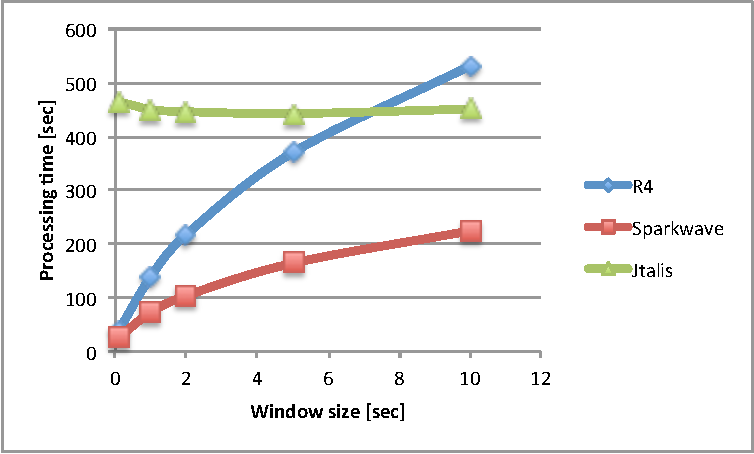
\includegraphics[width=0.45\textwidth]{all-systems-varying-windows.png}
		\caption{A comparison of the times taken by the systems R4, Sparkwave and ETALIS to process 1.1 million triples from a single input stream, given sliding windows of various sizes over the input stream.}
		\labelfig{all-systems-varying-windows}
	\end{figure}
	The X axis shows the time windows in milliseconds while the Y axis shows the processing time in milliseconds.
	Generally, R4 is faster than Etalis but slower than Sparkwave.
	The increasing difference between R4 and Sparkwave while increasing the window size is due to the fact that Sparkwave uses a hash join algorithm while the current implementation of R4 uses sequential joins, so as the beta memories (i.e time windows) grow bigger, the join needs significantly longer time to iterate over the windows in the matching process.
	More efficient join algorithms are considered in the mean time.

	Talk about Sparkwave limited exprisseviness?

%	\subimport{conclusions/}{future-work.tex}
\end{nestedsection}